\documentclass[12pt]{article}

% ----------------------------------------------------------------------
% Define external packages, language, margins, fonts, and new commands 
% and colors
% ----------------------------------------------------------------------
\usepackage[utf8]{inputenc} % Codification
\usepackage[english]{babel} % Writing idiom
\usepackage{pgfplots}
\pgfplotsset{compat=1.18}
\usepackage[export]{adjustbox} % Align images
\usepackage{amsmath} % Extra commands for math mode
\usepackage{amssymb} % Mathematical symbols
\usepackage{anysize} % Personalize margins
    \marginsize{2cm}{2cm}{2cm}{2cm} %{left}{right}{above}{below}
\usepackage{appendix} % Appendices
\usepackage{cancel} % Expression cancellation
\usepackage{caption} % Captions
    \DeclareCaptionFont{newfont}{\fontfamily{cmss}\selectfont}
    \captionsetup{labelfont={bf, newfont}}
\usepackage{cite} % Citations, like [1 - 3]
\usepackage{color} % Text coloring
\usepackage{fancyhdr} % Head note and footnote
    \pagestyle{fancy}
    \fancyhf{}
    \fancyhead[R]{\footnotesize \fontfamily{cmss}\selectfont Assignment 1} % Right of Head note
    \fancyfoot[L]{\footnotesize \fontfamily{cmss}\selectfont COL380} % Left of Footnote
    \fancyfoot[C]{\thepage} % Center of Footnote
    \fancyfoot[R]{\footnotesize \fontfamily{cmss}\selectfont Introduction to Distributed and Parallel Programming} % Right of Footnote
    \renewcommand{\footrulewidth}{0.4pt} % Footnote rule
\usepackage{float} % Utilization of [H] in figures
\usepackage{graphicx} % Figures in LaTeX
\usepackage[colorlinks = true, plainpages = true, linkcolor = istblue, urlcolor = istblue, citecolor = istblue, anchorcolor = istblue]{hyperref}
\usepackage{indentfirst} % First paragraph
\usepackage[super]{nth} % Superscripts
\usepackage{siunitx} % SI units
\usepackage{subcaption} % Subfigures
\usepackage{titlesec} % Font
    \titleformat{\section}{\fontfamily{cmss}\selectfont\Large\bfseries}{\thesection}{1em}{}
    \titleformat{\subsection}{\fontfamily{cmss}\selectfont\large\bfseries}{\thesubsection}{1em}{}
    \titleformat{\subsubsection}{\fontfamily{cmss}\selectfont\normalsize\bfseries}{\thesubsubsection}{1em}{}
    \fancyfoot[C]{\fontfamily{cmss}\selectfont\thepage}

% Random text (not needed)
\usepackage{lipsum}
\usepackage{duckuments}

% New and re-newcommands
\newcommand{\sen}{\operatorname{\sen}} % Sine function definition
\newcommand{\HRule}{\rule{\linewidth}{0.5mm}} % Specific rule definition
\renewcommand{\appendixpagename}{\LARGE \fontfamily{cmss}\selectfont Appendices}

% Colors
\definecolor{istblue}{RGB}{3, 171, 230}
\definecolor{dkgreen}{rgb}{0,0.6,0}
\definecolor{gray}{rgb}{0.5,0.5,0.5}

\begin{document}

% ----------------------------------------------------------------------
% Cover
% ----------------------------------------------------------------------
\begin{center}
    \begin{figure}
        \vspace{0.0cm}
        \includegraphics[scale = 0.3, center]{images/LOGO_IITD (1).jpeg} % IST logo
    \end{figure}
    \mbox{}\\[2.0cm]
    \vspace{-2.0cm}
    \textsc{\Huge COL380}\\[2.5cm]
    \textsc{\LARGE Introduction to Distributed and Parallel Programming}\\[2.0cm]
    \HRule\\[0.4cm]
    {\large \bf {\fontfamily{cmss}\selectfont Assignment 1\\Harnessing Threads: Efficient LU Decomposition with OpenMP and POSIX Threads} 
    }\\[0.2cm]
    \HRule\\[0.5cm]
\end{center}

\begin{flushleft}
    \textbf{\fontfamily{cmss}\selectfont Authors:}
\end{flushleft}

\begin{center}
    \begin{minipage}{0.5\textwidth}
        \begin{flushleft}
            Keval Makwana (2021CS10585)\\
            Dev Sutariya (2021CS10793) \\
            Ayushman Kumar Singh (2021CS51004)
        \end{flushleft}
    \end{minipage}%
    \begin{minipage}{0.5\textwidth}
        \begin{flushright}
            \href{mailto:cs1210585@cse.iitd.ac.in}{\texttt{cs1210585@cse.iitd.ac.in}}\\
            \href{mailto:cs1210793@cse.iitd.ac.in}
            {\texttt{cs1210793@cse.iitd.ac.in}} \\
            \href{mailto:cs5211004@cse.iitd.ac.in}{\texttt{cs5211004@cse.iitd.ac.in}}
        \end{flushright}
    \end{minipage}
\end{center}
\vspace{0.5 cm}

\begin{flushleft}
    \textbf{\fontfamily{cmss}\selectfont Instructor:}
\end{flushleft}

\vspace{-0.5 cm}

\begin{flushleft}
    \fontfamily{cmss}\selectfont  Rijurekha Sen                 
\end{flushleft}

\begin{flushleft}
    \large {\text{\bf \fontfamily{cmss}\selectfont } }\\[4.0cm]
\end{flushleft}
\vspace{-2.0cm}    
\begin{center}
    \large \bf \fontfamily{cmss}\selectfont 2023/2024 -- \nth{2} Semester
\end{center}

\thispagestyle{empty}

\setcounter{page}{0}

\newpage

% ----------------------------------------------------------------------
% Contents
% ----------------------------------------------------------------------
\tableofcontents 
\setcounter{page}{1}
\newpage

% ----------------------------------------------------------------------
% Body
% ----------------------------------------------------------------------
\section{Brief Introduction to Problem Statement}
\paragraph{The aim of this assignment is to develop efficient parallel implementations of LU decomposition with row pivoting, a core algorithm in linear algebra with widespread applications in scientific computing. This assignment explores two shared-memory parallel programming paradigms: \textbf{OpenMP} and \textbf{Pthreads} (POSIX Threads). The core objectives are: }
\begin{itemize}
    \item \textbf{Implementation: }Construct correct parallel implementations of LU decomposition with row pivoting in both \verb|OpenMP| and \verb|Pthreads| framework.
    \item \textbf{Verification: }Ensure the correctness of the parallel implementations by calculating the residual matrix (PA - LU) and its L2,1 norm. A small norm value serves as a quantitative measure of the implementation's accuracy.
    \item \textbf{Performance Optimization:} Enhance the parallel implementations by carefully managing work partitioning, synchronization, data layout, and addressing potential issues like false sharing.
    \item \textbf{Comparative Analysis: }Evaluate the performance of both implementations across various thread counts. Analyze their scaling behaviour and parallel efficiency, identifying factors that contribute to performance gains or limitations.
\end{itemize}

\section{Sequential Algorithm Overview}
Here is a detailed overview of the LU decomposition algorithm with row pivoting:
\begin{enumerate}
    \item \textbf{Initialization:}
    \begin{itemize}
        \item Create matrices: \verb|a| (the input matrix), \textbf{$\pi$} (permutation vector), \verb|l| (lower triangular matrix), \verb|u| (upper triangular matrix).
        \item Initialize \verb|l| as an identity matrix, \verb|u| with zeros below the diagonal, and \textbf{$\pi$} with sequential indices.
    \end{itemize}
    \item \textbf{Iteration and Pivoting}
    \begin{verbatim}
        for k = 1 to n
        max = 0
        for i = k to n
            if max < |a(i,k)|
            max = |a(i,k)|
            k' = i
        if max == 0
            error (singular matrix)
        swap pi[k] and pi[k']
        swap a(k,:) and a(k',:)
        swap l(k,1:k-1) and l(k',1:k-1)
        u(k,k) = a(k,k)
        for i = k+1 to n
            l(i,k) = a(i,k)/u(k,k)
            u(k,i) = a(k,i)
        for i = k+1 to n
            for j = k+1 to n
                a(i,j) = a(i,j) - l(i,k)*u(k,j)|
    \end{verbatim}
\end{enumerate}

\section{Analysing Sequential Algorithm}
\paragraph{During the analysis of the sequential code, we identified regions where parallelization can be beneficial.}
\paragraph{The outer "for" loop should be excluded from parallelization due to existing data dependencies, each step (k) relies on the completion of the previous step (k-1).}
\paragraph{Within the outer loop, the double-for loop is responsible for updating elements in the residual matrix. Since, these updates are independent, parallelization can be used to enhance efficiency.}
\paragraph{Moreover, row-swapping operations, involving the swapping of elements at specific indices, can be parallelized.}
\paragraph{Each swap operation at a given index is independent of other indices, enabling parallel execution.}

\section{Analysing OpenMP Implementation}
\begin{enumerate}
    \item \textbf{Finding Maximum Element in Column:}
    \begin{itemize}
        \item The loop finding the maximum absolute value in the k-th column is parallelized using OpenMP's reduction clause to find the maximum value across threads efficiently.
    \end{itemize}
    \item \textbf{Permutation Index Swap:}
    \begin{itemize}
        \item The permutation indices (`\textbf{pi}`) are swapped to keep track of row permutations in parallel.
    \end{itemize}
    \item \textbf{Parallel Row Swapping:}
    \begin{itemize}
        \item The rows in the matrix `\textbf{a}` are swapped in parallel, improving performance by distributing the work across threads.
    \end{itemize}
    \item \textbf{Parallel Lower Triangular Matrix Swap:}
    \begin{itemize}
        \item Elements in the lower triangular matrix `\textbf{l}` are swapped in parallel, ensuring consistency with the row swaps in the matrix `\textbf{a}`.
    \end{itemize}
    \item \textbf{Assigning Diagonal Element:}
    \begin{itemize}
        \item The diagonal element of the upper triangular matrix `\textbf{u}` is assigned. This step is not parallelized as it involves a single assignment.
    \end{itemize}
    \item \textbf{Parallel Updating of Lower and Upper Matrices:}
    \begin{itemize}
        \item Sections updating the lower and upper matrices (`\textbf{l}` and `\textbf{u}`) are parallelized, improving efficiency by utilizing multiple threads.
    \end{itemize}
    \item \textbf{Parallel Update of Matrix a:}
    \begin{itemize}
        \item The remaining elements in the matrix `\textbf{a}` are updated in parallel. This section is collapsed into a 2D loop for parallelization across both dimensions.
    \end{itemize}
\end{enumerate}

\begin{figure}[ht]
  \centering
  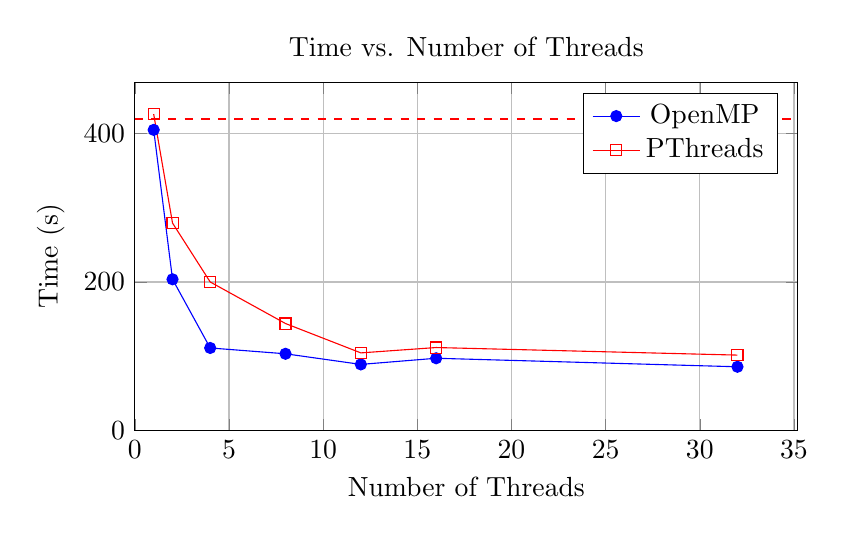
\begin{tikzpicture}
    \begin{axis}[
      title={Time vs. Number of Threads},
      xlabel={Number of Threads},
      ylabel={Time (s)},
      xmin=0,
      ymin=0,
      grid=major,
      legend pos=north east,
      width=10cm,
      height=6cm,
      ]
      
      \addplot[mark=*, blue] coordinates {
        (1, 404.894)
        (2, 203.599)
        (4, 111.085)
        (8, 103.232)
        (12, 88.9214)
        (16, 97.2119)
        (32, 85.7303)
      };
      \addlegendentry{OpenMP}

      \addplot[mark=square, red] coordinates {
        (1, 426.127)
        (2, 279.37)
        (4, 200.005)
        (8, 144.001)
        (12, 104.447)
        (16, 111.658)
        (32, 101.463)
      };
      \addlegendentry{PThreads}

      \draw[red, dashed] (axis cs:0, 419.571) -- (axis cs:35, 419.571);
      \addlegendentry{Sequential Time}


    \end{axis}
  \end{tikzpicture}
  \caption{Performance Comparison}
  \label{fig:time_vs_threads}
\end{figure}

\end{document}



